\chapter{Specifikacija programske potpore}
		
	\section{Funkcionalni zahtjevi}
			
		
			
			
			\noindent \textbf{Dionici:}
			
			\begin{packed_enum}
				
				\item Vježbači
				\item Treneri			
				\item Administrator
				\item Baza podataka
				
			\end{packed_enum}
			
			\noindent \textbf{Aktori i njihovi funkcionalni zahtjevi:}
			
			
			\begin{packed_enum}
				\item  \underbar{Neregistrirani/neprijavljeni korisnik može:}
				
				\begin{packed_enum}
					
					\item se registrirati u sustav, stvoriti novi korisnički račun za koji su mu potrebni korisničko ime, lozinka, ime, prezime, broj mobitela, e-mail adresa, datum rođenja, uloga, cilj (ovisno o ulozi)
				
					
				\end{packed_enum}
			
				\item  \underbar{Vježbač (primarni dionik) može:}
				
				\begin{packed_enum}
					
					\item pregledavati i mijenjati osobne podatke
					\item birati i rezervirati određenu vrstu treninga u skladu sa postavljenim ciljevima
     				\item otkazivati rezervacije
					\item odabrati željeni fitness cilj
					\item mijenjati ciljeve završetkom tekućeg mjeseca
					
				\end{packed_enum}
				
				\item  \underbar{Trener (primarni dionik) može:}
				
				\begin{packed_enum}
					
					\item određivati vrstu treninga po terminima
					\item napraviti raspored treninga prema određenim ciljevima vježbača
					\item na temelju fonda sati koji je odabrao vježbač odrediti koliko različitih vrsta treninga vježbač mora odraditi
					\item izraditi trening
					\item za vrste treninga napisati vlastita pravila
					\item definirati maksimalan broj polaznika za određenu vrstu treninga
					
				\end{packed_enum}
				
				
				\item  \underbar{Administrator (sekundarni dionik) može:}
				
				\begin{packed_enum}
					
					\item vidjeti popis svih registriranih korisnika i njihovih osobnih podataka
					\item verificirati račune trenera
					\item brisati korisničke račune
				
					
				\end{packed_enum}
				
				
				\item  \underbar{Baza podataka (sudionik) može:}
				
				\begin{packed_enum}
					
					\item pohranjuje sve podatke o korisnicima i njihovim ovlastima
					\item pohranjuje sve podatke o treninzima, vježbama, terminima i njihovim opisima i ograničenjima
				
					
				\end{packed_enum}
				
			\end{packed_enum}
			
			\eject 
			
			
				
			\subsection{Obrasci uporabe}
				
				%\textbf{\textit{dio 1. revizije}}
				
				\subsubsection{Opis obrazaca uporabe}
					
					\noindent \underbar{\textbf{UC1 - Registriraj korisnika}}
					\begin{packed_item}
	
						\item \textbf{Glavni sudionik: } Neregistrirani korisnik
						\item  \textbf{Cilj:} Izrada korisničkog računa
						\item  \textbf{Sudionici:} Baza podataka
						\item  \textbf{Preduvjet:} Pristup aplikaciji putem web preglednika
						\item  \textbf{Opis osnovnog tijeka:}
						
						\item[] \begin{packed_enum}
							
							\item Neregistrirani korisnik bira opciju "Registriraj se"
       					\item Sustav otvara formu za upis podataka
							\item Neregistrirani korisnik unosi potrebne podatke (matični i kontakt podatci)
							\item Neregistrirani korisnik odabire tip registracije (klijent ili trener)
							\begin{packed_enum}
							    \item Neregistrirani korisnik odabire tip registracije \textit{trener} i sustav preskače korak 5.
							    \item Neregistrirani korisnik odabire tip registracije \textit{klijent}
							\end{packed_enum}
							
							\item Neregistrirani korisnik odabire cilj
							
                            \item Neregistrirani korisnik odabire gumb "Registriracija"
							\item Sustav provjerava i utvrđuje dostupnost korisničkog imena i maila te ispravnost ostalih unesenih podataka u skladu s zahtjevima sustava
							\item Sustav na upisani mail šalje se link za aktivaciju korisničkog računa
                            \item Sustav pohranjuje potvrdu maila, aktivira korisnički račun i obavještava korisnika o uspješnoj registraciji
                            \item Sustav preusmjerava registriranog korisnika na stranicu "Prijava"
							
						\end{packed_enum}
						
						\item  \textbf{Opis mogućih odstupanja:}
						
						\item[] \begin{packed_item}

      					\item[6.a] Neregistrirani korisnik odustaje od registracije
							\item[] \begin{packed_enum}
								
								\item Neregistriranog se korisnika preusmjerava na početnu stranicu
								
							\end{packed_enum}
	
							\item[7.a] Sustav je provjerio i utvrdio da je neregistrirani korisnik unio neispravan oblik mail adrese, email već postoji u bazi podataka, unio je korisničko ime koje se već koristi ili je unio lozinku u nedozvoljene duljine
							\item[] \begin{packed_enum}
								
								\item Sustav obavještava neregistriranog korisnika o pogreškama te se izvođenje tijeka nastavlja u koraku 4.
								
							\end{packed_enum}

						\end{packed_item}
					\end{packed_item}
     
					\noindent \underbar{\textbf{UC2 - Prijavi korisnika}}
					\begin{packed_item}
	
						\item \textbf{Glavni sudionik: }Korisnik
						\item  \textbf{Cilj:} Prijava u sustav
						\item  \textbf{Sudionici:} Baza podataka, korisnik
						\item  \textbf{Preduvjet:} Pristup aplikaciji putem web preglednika
						\item  \textbf{Opis osnovnog tijeka:}
						
						\item[] \begin{packed_enum}
							\item Korisnik bira opciju "Prijava"  
       					\item Sustav otvara formu za upis podataka
							\item Korisnik upisuje svoje korisničko ime i lozinku
                            \item Korisnik odabire potvrdu aplikacije
							\item Sustav provjerava i utvrđuje postojanje i ispravnost podataka unesenih u formu
                            \item Sustav obavještava korisnika o uspješnoj prijavi
                            \item Sustav preusmjerava korisnika na glavnu stranicu
							\item Korisnik dobiva pristup korisničkim funkcijama ovisnima o ulozi

						\end{packed_enum}
						
						\item  \textbf{Opis mogućih odstupanja:}
						
						\item[] \begin{packed_item}
      					\item[4.a] Korisnik odustaje od prijave
       
						\item[5.a] Sustav je provjerio i utvrdio da je korisnik upisao neispravno korisničko ime i/ili lozinku ili račun nije verificiran putem maila i/ili od strane administratora (za slučaj prijave trenera)
							\item[] \begin{packed_enum}
								
								\item Sustav obavještava korisnika o pogreškama te se izvođenje tijeka nastavlja u koraku 4.					
							\end{packed_enum}
                        \end{packed_item}
                    \end{packed_item}

					\noindent \underbar{\textbf{UC3 - Odjavi korisnika}}
					\begin{packed_item}
	
						\item \textbf{Glavni sudionik: } Korisnik
						\item  \textbf{Cilj:} Odjavljivanje korisnika iz sustava
						\item  \textbf{Sudionici:} Baza podataka
						\item  \textbf{Preduvjet:} Korisnik mora biti prijavljen u sustav
						\item  \textbf{Opis osnovnog tijeka:}
						
						\item[] \begin{packed_enum}
	
							\item Prijavljeni korisnik bira opciju "Odjava"
							\item Sustav prijavljenom korisniku prikazuje prozor za potvrdu odjave
							\item Korisnik potvrđuje odjavu klikom 
							\item Sustav odjavljuje korisnika
							\item Sustav preusmjerava korisnika na stranicu za prijavu
							
						\end{packed_enum}
						\item  \textbf{Opis mogućih odstupanja:}
						
						\item[] \begin{packed_item}
	
							\item[3.a] Prijavljeni korisnik odustaje od odjave
							\item[] \begin{packed_enum}

                                \item Sustav zatvara prozor za potvrdu odjave iz sustava
								
                
								
							\end{packed_enum}
							
						\end{packed_item}
						
					\end{packed_item}
     
					\noindent \underbar{\textbf{UC4 - Pregledaj korisničke podatke}}
					\begin{packed_item}
	
						\item \textbf{Glavni sudionik: }Korisnik
						\item  \textbf{Cilj:} Pregled osobnih podataka
						\item  \textbf{Sudionici:} Baza podataka
						\item  \textbf{Preduvjet:} Korisnik je prijavljen u sustav
						\item  \textbf{Opis osnovnog tijeka:}
						
						\item[] \begin{packed_enum}
							\item Prijavljeni korisnik bira opciju ”Osobni podatci”
                            \item Sustav preusjerava prijavljenog korisnika na stranicu "Osobni podatci"
                            \item Sustav učitava iz baze podataka osobne podatke prijavljenog korisnika(matični i kontakt podatci)
                            \item Sustav prikazuje učitane podatke na stranici
                            \item Korisnik pregledava prikazane podatke
						\end{packed_enum}
                        
                    \end{packed_item}	
                    
					\noindent \underbar{\textbf{UC5 - Promijeni korisničke podatke}}
					\begin{packed_item}
	
						\item \textbf{Glavni sudionik: }Korisnik
						\item  \textbf{Cilj:} Promjena osobnih podataka
						\item  \textbf{Sudionici:} Baza podataka
						\item  \textbf{Preduvjet:} Korisnik je prijavljen u sustav
						\item  \textbf{Opis osnovnog tijeka:}
						
						\item[] \begin{packed_enum}
	
							\item Korisnik odabire opciju ”Promjena podataka”
       					\item Sustav otvara formu za promjenu podataka
                            \item Prijavljeni korisnik mijenja podatke po želji
                            \item Prijavljeni korisnik odabire potvrdu aplikacije
                            \item Sustav provjerava i utvrđuje jesu li novi podatci ispravnog oblika
                            \item Sustav pohranjuje nove podatke u bazu podataka
                            \item Sustav obavještava prijavljenog korisnika o uspješnoj promjeni                           
                            \end{packed_enum}
						
	                \item  \textbf{Opis mogućih odstupanja:}
                    \item[] \begin{packed_item}
							\item[4.a] Prijavljeni korisnik je odustao od promjene
							\item[] \begin{packed_enum}
								
								\item Sustav preusmjerava prijavljenog korisnika na stranicu "Osobni podatci"				
							\end{packed_enum}
                            \item[5.a] Sustav je utvrdio da uneseni podatci nisu ispravnog formata
							\item[] \begin{packed_enum}
								
								\item Sustav obavještava prijavljenog korisnika o pogreškama te se izvođenje tijeka nastavlja u koraku 3.					
							\end{packed_enum}
                        \end{packed_item}
                    \end{packed_item}

					\noindent \underbar{\textbf{UC6 - Obriši korisnički račun}}
					\begin{packed_item}
	                   
						\item \textbf{Glavni sudionik: } Admin
						\item  \textbf{Cilj:} Brisanje korisničkog računa iz baze podataka
						\item  \textbf{Sudionici:} Baza podataka
						\item  \textbf{Preduvjet:} Administrator mora biti prijavljen u sustav
						\item  \textbf{Opis osnovnog tijeka:}
						
						\item[] \begin{packed_enum}
	
							\item Adminstrator bira opciju "Obriši korisnički račun"
							\item Administratoru se prikazuje prozor u kojem potvrđuje brisanje korisničkog računa
                            \item Administrator odabire potvrdu aplikacije
							\item Sustav briše račun iz baze podataka
							\item Sustav obavještava administratora o uspješnom brisanju računa
							\item Sustav obavještava korisnika o brisanju računa
							
						\end{packed_enum}
						\item  \textbf{Opis mogućih odstupanja:}
						\item[] \begin{packed_item}
	
							\item[3.a] Administrator odustaje od brisanja računa
							\item[] \begin{packed_enum}

                                \item Zatvaranje prozora za potvrdu brisanja računa iz sustava

							\end{packed_enum}
							
						\end{packed_item}
      
					\end{packed_item}

					\noindent \underbar{\textbf{UC7 - Promijeni cilj}}
					\begin{packed_item}
	
						\item \textbf{Glavni sudionik: }Klijent
						\item  \textbf{Cilj:} Odabir cilja sudjelovanja u programu vježbanja
						\item  \textbf{Sudionici:} Baza podataka
						\item  \textbf{Preduvjet:} Zadnji je tjedan tekućeg mjeseca
						\item  \textbf{Opis osnovnog tijeka:}

						
						\item[] \begin{packed_enum}
	
							\item Klijent bira opciju "Promjena cilja"
							\item Sustav prikazuje klijentu ciljeve koje može odabrati
                            \item Klijent odabire cilj koji želi
							\item Klijent odabire potvrdu aplikacije
       					\item Sustav pohranjuje odabrani cilj
       					\item Sustav uklanja klijenta iz liste klijenata trenera te uklanja sve dodijeljene treninge klijentu zbog promjene cilja
       					\item Sustav obavještava klijenta o uspješnoj promjeni cilja
						\item Klijenta se preusmjerava na glavnu stranicu
							
						\end{packed_enum}
						\item  \textbf{Opis mogućih odstupanja:}
						\item[] \begin{packed_item}
	
							\item[4.a] Klijent odustaje od promjene cilja
							\item[] \begin{packed_enum}

                                \item Sustav preusmjerava klijenta na glavnu stranicu

								
							\end{packed_enum}
							
						\end{packed_item}
      
					\end{packed_item}
						

					\noindent \underbar{\textbf{UC8 - Izradi trening}}
					\begin{packed_item}
	
						\item \textbf{Glavni sudionik: }Trener
						\item  \textbf{Cilj:} Izrada treninga
						\item  \textbf{Sudionici:} Baza podataka
						\item  \textbf{Preduvjet:} Trener mora biti prijavljen u sustav
						\item  \textbf{Opis osnovnog tijeka:}
						
						\item[] \begin{packed_enum}
	
							\item Trener bira opciju "Izradi trening"
							\item Sustav otvara prozor za izradu treninga s formom za unos podataka o treningu
							\item Trener unosi glavne podatke o treningu
       					\item Trener odabire dane u tjednu u kojima bi se izvodio trening
							\item Sustav za svaki dan nudi opciju odabira slobodnog tremina
							\item Trener odabire po jedan termin za svaki odabrani dan
							\item Trener odabire opciju "Potvrdi" unutar forme
                            \item Sustav provjerava jesu li podaci ispravnog oblika
                            \item Sustav pohranjuje podatke o treningu i njegovim treminima u bazu podataka
                            \item Sustav obavještava trenera o uspješno unesenom treningu
                            \item Sustav preusmjerava trenera na stranicu svih njegovih treninga
						\end{packed_enum}
						
						\item  \textbf{Opis mogućih odstupanja:}
						
						\item[] \begin{packed_item}
	
							\item[8.a] Trener odustaje od izrade treninga
							\item[] \begin{packed_enum}
								
								\item Trenera se preusmjerava na stranicu svih njegovih treninga
								
								
							\end{packed_enum}
							\item[9.a] Sustav je utvrdio da je trener unio neispravan oblik podataka o treningu
							\item[] \begin{packed_enum}
								
								\item Sustav obavještava trenera o pogreškama te se izvođenje nastavlja od koraka 4.
								
								
							\end{packed_enum}							
							
						\end{packed_item}
					\end{packed_item}

					

					

				

				    \noindent \underbar{\textbf{UC9 - Pregledaj klijenate kojima nisu dodijeljeni treninzi }}
					\begin{packed_item}
	
						\item \textbf{Glavni sudionik: } Trener
						\item  \textbf{Cilj:} Dobiti uvid u klijente kojima nije dodijeljen trening
						\item  \textbf{Sudionici:} Baza podataka
						\item  \textbf{Preduvjet:} Trener je prijavljen u sustav
						\item  \textbf{Opis osnovnog tijeka:}
						
						\item[] \begin{packed_enum}
	                        
							\item Trener odabire opciju "Prikaži klijente bez dodijeljenog treninga"
							\item Sustav dohvaća podatke iz baze podataka o klijentima bez dodijeljenog treninga
							\item Sustav prikazuje dohvaćene podatke o klijentima na stranici
							\item Trener pregledava prikazane klijente
							
							
						\end{packed_enum}
						
					
					\end{packed_item}
    



					\noindent \underbar{\textbf{UC10 - Dodijeli treninge klijentu}}
					\begin{packed_item}
	
						\item \textbf{Glavni sudionik: }Trener
						\item  \textbf{Cilj:} Dodjela treninga klijentu
						\item  \textbf{Sudionici:} Baza podataka, klijent
						\item  \textbf{Preduvjeti:} Klijent je registriran u sustav, trener je priavljen u sustav
						\item  \textbf{Opis osnovnog tijeka:}
						
						\item[] \begin{packed_enum}
	
						\item Trener odabire klijenta sa stranice "Prikaz klijenata bez dodijeljenog treninga"
						
                            \item Treneru se za dodjelu prikazuju svi mogući treninzi sa opcijom "Dodijeli"
                            \item Trener odabire treninge za dodjelu opcijom "Dodijeli"
                            \item Trener unosi broj sati predviđenih za odrađivanje odabranih treninga klijenta na mjesečnoj bazi
						\item Trener potvrđuje dodijeljene treninge i unos odabirom opcije "Spremi"
						\item Sustav ispituje ispravnost spremljenih podataka
                            \item Sustav sprema dodijeljene treninge i broj sati u bazu podataka
                            \item Sustav obavještava trenera o uspješno dodijeljenim treninzima
                            \item Sustav obavještava klijenta o dodijeljenim treninzima putem emaila
                            
						\end{packed_enum}
						
						\item  \textbf{Opis mogućih odstupanja:}
						
						\item[] \begin{packed_item}

      						\item[6.a] Sustav je utvrdio da trener nije odabrao ni jedan trening i/ili unio broj sati
							\item[] \begin{packed_enum}
								
								\item Sustav ne sprema promjene, tj. ne evidentira klijenta kao onog kojemu su dodijeljeni treninzi te se izvođenje nastavlja u koraku 1.					
							\end{packed_enum}
	
							\item[5.a] Trener nije potvrdio dodijeljene treninge i/ili unio broj sati
							\item[] \begin{packed_enum}
								
								\item Sustav obavještava trenera o nespremljenim promjenama te se izvođenje nastavlja u koraku 1.
							\end{packed_enum}
                        \end{packed_item}
                    \end{packed_item}
                    

					
					\noindent \underbar{\textbf{UC11 - Pregledaj termine dodijeljenih treninga}}
					\begin{packed_item}
	
						\item \textbf{Glavni sudionik: } Klijent
						\item  \textbf{Cilj:} Pregledati dodijeljene treninge i termine
						\item  \textbf{Sudionici:} Baza podataka
						\item  \textbf{Preduvjet:} Klijent je na stranici "Pregled dodijeljenih treninga"
						\item  \textbf{Opis osnovnog tijeka:}
						
						\item[] \begin{packed_enum}
	                        
							\item Klijent odabire trening sa stranice "Pregled dodijeljenih treninga"
							\item Sustav dohvaća termine odabranog treninga iz baze podataka
							\item Sustav prikazuje klijentu termine odabranog treninga
							\item Klijent pregledava termine prikazanog treninga
							
							
						\end{packed_enum}
						
						
					\end{packed_item}

   					\noindent \underbar{\textbf{UC12 - Rezerviraj termin dodijeljenog treninga}}
					\begin{packed_item}
	
						\item \textbf{Glavni sudionik: } Klijent
						\item  \textbf{Cilj:} Rezervirati termin treninga
						\item  \textbf{Sudionici:} Baza podataka
						\item  \textbf{Preduvjet:} Klijent mora imati dodijeljen trening
						\item  \textbf{Opis osnovnog tijeka:}
						
						\item[] \begin{packed_enum}
							\item Klijent je na stranici "Moji treninzi"      
							\item Klijent odabire termin među ponuđenima
							\item Klijent klikom na gumb "Rezerviraj" rezervira termin
							\item Sustav otvara prozor u kojem traži potvrdu rezervacije termina
							\item Klijent odabire potvrdu aplikacije
							\item Sustav provjerava ograničenja sustava
							\item Sustav unosi podatak o rezervaciji u bazu podataka
							\item Sustav smanjuje fond sati klijenta za jedan
							\item Sustav smanjuje broj raspoloživih mjesta u rezervaciji treninga za jedan
							\item Sustav obavještava klijenta o uspješnoj rezervaciji
							
							
						\end{packed_enum}
						
						\item  \textbf{Opis mogućih odstupanja:}
						
						\item[] \begin{packed_item}

							\item[5.a] Klijent odustaje od rezervacije
							\item[] \begin{packed_enum}
								
								\item Klijent je preusmjeren na stranicu prikaza svih termina njemu dodijeljenih treninga
								
							\end{packed_enum}
	
							\item[6.a] Sustav je utvrdio da rezervacija nije u skladu s ograničenjima sustava
							\item[] \begin{packed_enum}
								
								\item Sustav obavještava klijenta da rezervaciju nije moguće izvršiti zbog ograničenja sustava te se izvođenje nastavlja od koraka 1.
								
							\end{packed_enum}
							
								
							
							
						\end{packed_item}
					\end{packed_item}
					\noindent \underbar{\textbf{UC13 - Otkaži rezervaciju termina treninga}}
					\begin{packed_item}
	
						\item \textbf{Glavni sudionik: } Klijent
						\item  \textbf{Cilj:} Otkazati rezervaciju
						\item  \textbf{Sudionici:} Baza podataka
						\item  \textbf{Preduvjet:} 
						\item  \textbf{Opis osnovnog tijeka:}
						
						\item[] \begin{packed_enum}
	                        
							\item Klijent je na stranici "Pregled dodijeljenih treninga"
							\item Klijent odabire trening koji želi otkazati
							\item Klijent klikom na gumb "Otkaži" otkazuje rezervaciju
							\item Sustav otvara prozor u kojem traži potvrdu otkaza rezervacije od klijenta
							\item Klijent odabire potvrdu aplikacije
							\item Sustav briše rezervaciju iz baze podataka
							\item Sustav povećava fond sati klijenta za jedan
							\item Sustav povećava broj mjesta treninga u odabranom terminu za jedan
							\item Sustav obavještava klijenta o uspješno otkazanoj rezervaciji
							
							
						\end{packed_enum}
						\item  \textbf{Opis mogućih odstupanja:}
						\item[] \begin{packed_item}
	
							\item[5.a] Klijent odustaje od otkaza rezervacije
							\item[] \begin{packed_enum}
								
								\item Klijent je preusmjeren na stranicu prikaza svojih rezervacija
								
							\end{packed_enum}
							
								
							
							
						\end{packed_item}						
						
					\end{packed_item}
                    \noindent \underbar{\textbf{UC14 - Pregledaj rezervacije}}
					\begin{packed_item}
	
						\item \textbf{Glavni sudionik: } Klijent
						\item  \textbf{Cilj:} Pregledati rezervirane termine treninga
						\item  \textbf{Sudionici:} Baza podataka
						\item  \textbf{Preduvjet:} 
						\item  \textbf{Opis osnovnog tijeka:}
						
						\item[] \begin{packed_enum}
	                        
							\item Klijent odabire opciju "Pregled rezervacija"
							\item Sustav dohvaća rezervacije termina trenutnog klijenta iz baze podataka
							\item Sustav prikazuje klijentu rezervacije termina treninga
							\item Klijent pregledava prikazane rezervacije
							
							
						\end{packed_enum}
						
						
					\end{packed_item}
					\noindent \underbar{\textbf{UC15 - Pregledaj sve korisničke račune}}
					\begin{packed_item}
	
						\item \textbf{Glavni sudionik: } Administrator
						\item  \textbf{Cilj:} Pregledati sve korisničke račune
						\item  \textbf{Sudionici:} Baza podataka
						\item  \textbf{Preduvjet:} Administrator mora biti prijavljen
						\item  \textbf{Opis osnovnog tijeka:}
						
						\item[] \begin{packed_enum}
	                        
							\item Administrator odabire opciju "Pregled svih korisničkih računa"
							\item Sustav preusmjerava administratora na stranicu pregleda računa   
							\item Sustav učitava sve račune iz baze podataka
							\item Sustav prikazuje administratoru račune s oznakom tipa računa (klijent, trener) i opcijom "Odobri" pored računa trenera
							\item Administrator pregledava prikazane račune
							
						\end{packed_enum}
						
						
					\end{packed_item}
					
					

					\noindent \underbar{\textbf{UC16 - Verificiraj novoregistrirane trenere}}
					\begin{packed_item}
	
						\item \textbf{Glavni sudionik: } Administrator
						\item  \textbf{Cilj:} Verifikacija  novoregistriranih trenera
						\item  \textbf{Sudionici:} Baza podataka
						\item  \textbf{Preduvjet:} Administrator mora biti prijavljen
						\item  \textbf{Opis osnovnog tijeka:}
						
						\item[] \begin{packed_enum}
	                        
							\item Administrator je na stranici "Pregled svih korisničkih računa"
							\item Sustav učitava sve korisničke račune 
							\item Administrator odabire trenera kojeg želi odobriti
							\item Administrator obabire gumb "Odobri"
							\item Sustav otvara prozor u kojem traži potvrdu administratora
							\item Administrator odabire potvrdu sustava
							\item Sustav ažurira bazu podataka
							\item Sustav obavještava administratora o uspješnoj verifikaciji
							
						\end{packed_enum}
						
						\item  \textbf{Opis mogućih odstupanja:}
						\item[] \begin{packed_item}
	
							\item[4.a] Administrator odustaje od verifikacije trenera
							\item[] \begin{packed_enum}
								
								\item Administrator je preusmjeren na stranicu "Pregled svih korisničkih računa"
								
							\end{packed_enum}
							
								
							
							
						\end{packed_item}						
					\end{packed_item}
					
				\subsubsection{Dijagrami obrazaca uporabe}
					
					\begin{figure}[H]
                      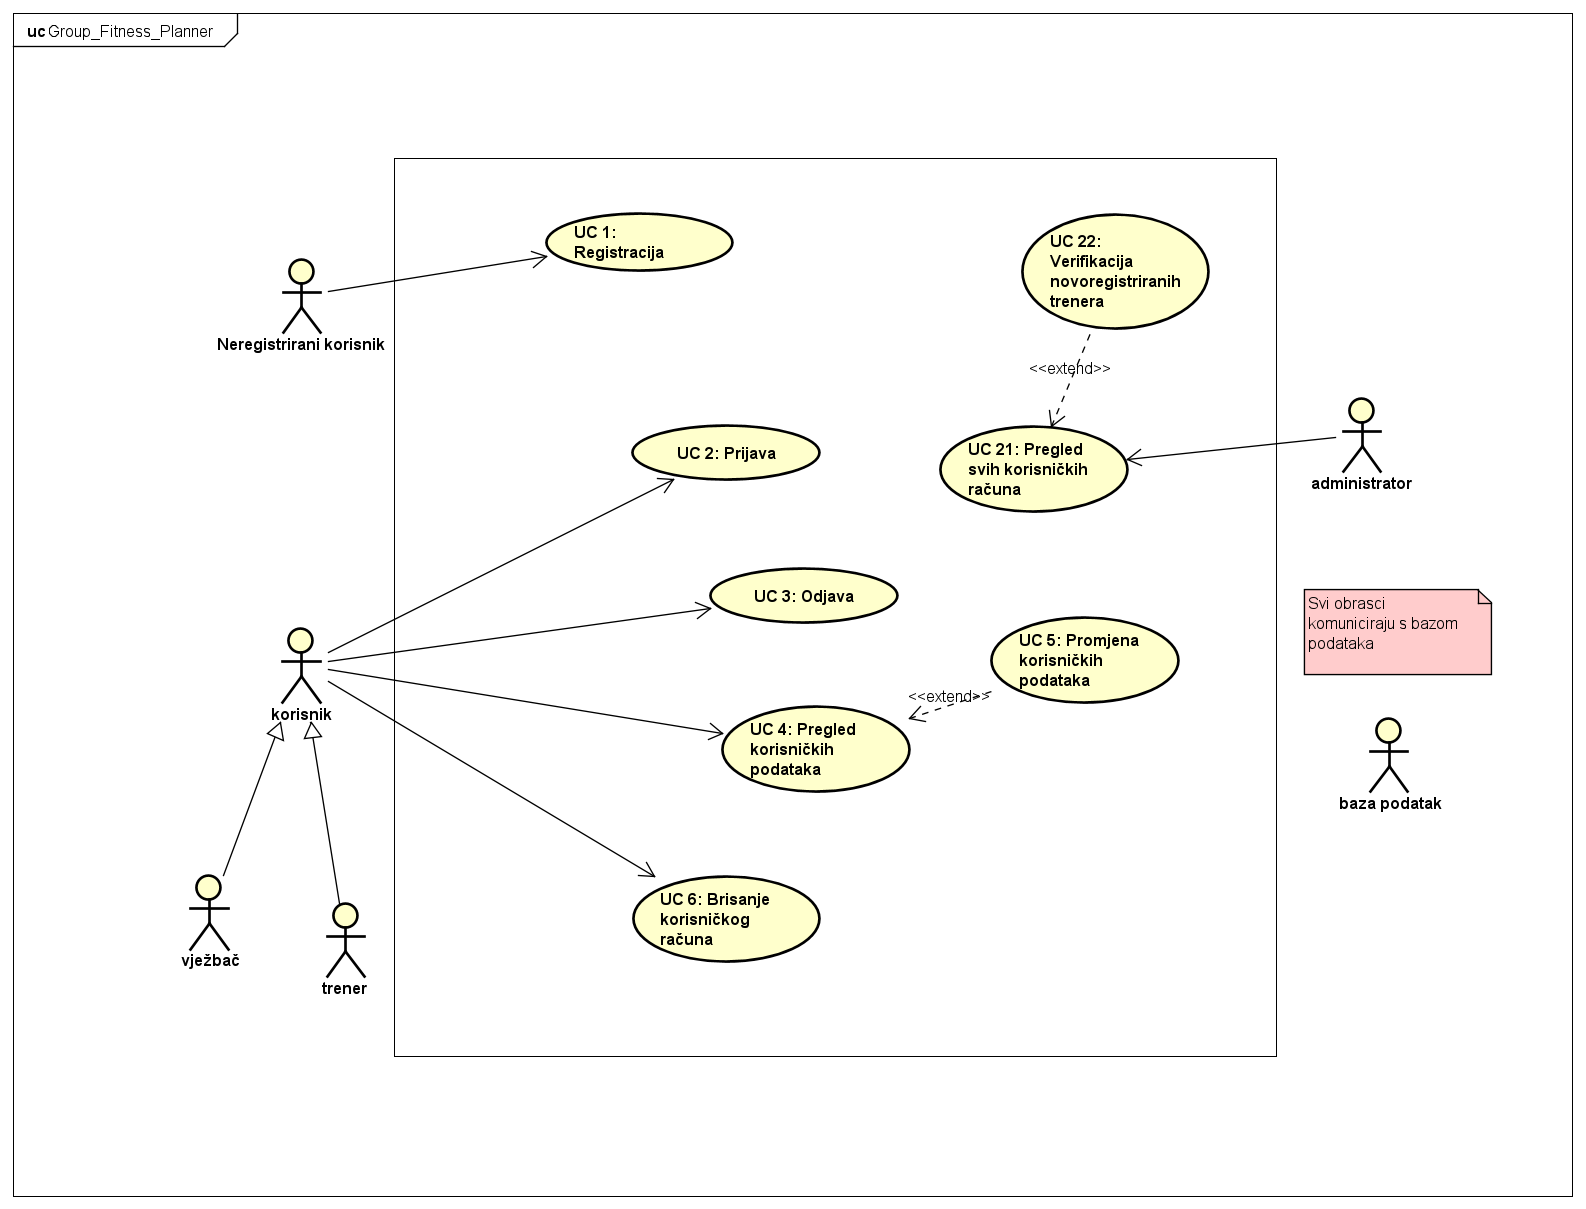
\includegraphics[scale=0.4]{./Dijagrami/UC0_Group_Fitness_Planner.png}
                      \centering
                      \caption{Dijagram obrasca uporabe}
                      \label{fig:promjene}
                \end{figure}
                \begin{figure}[H]
                      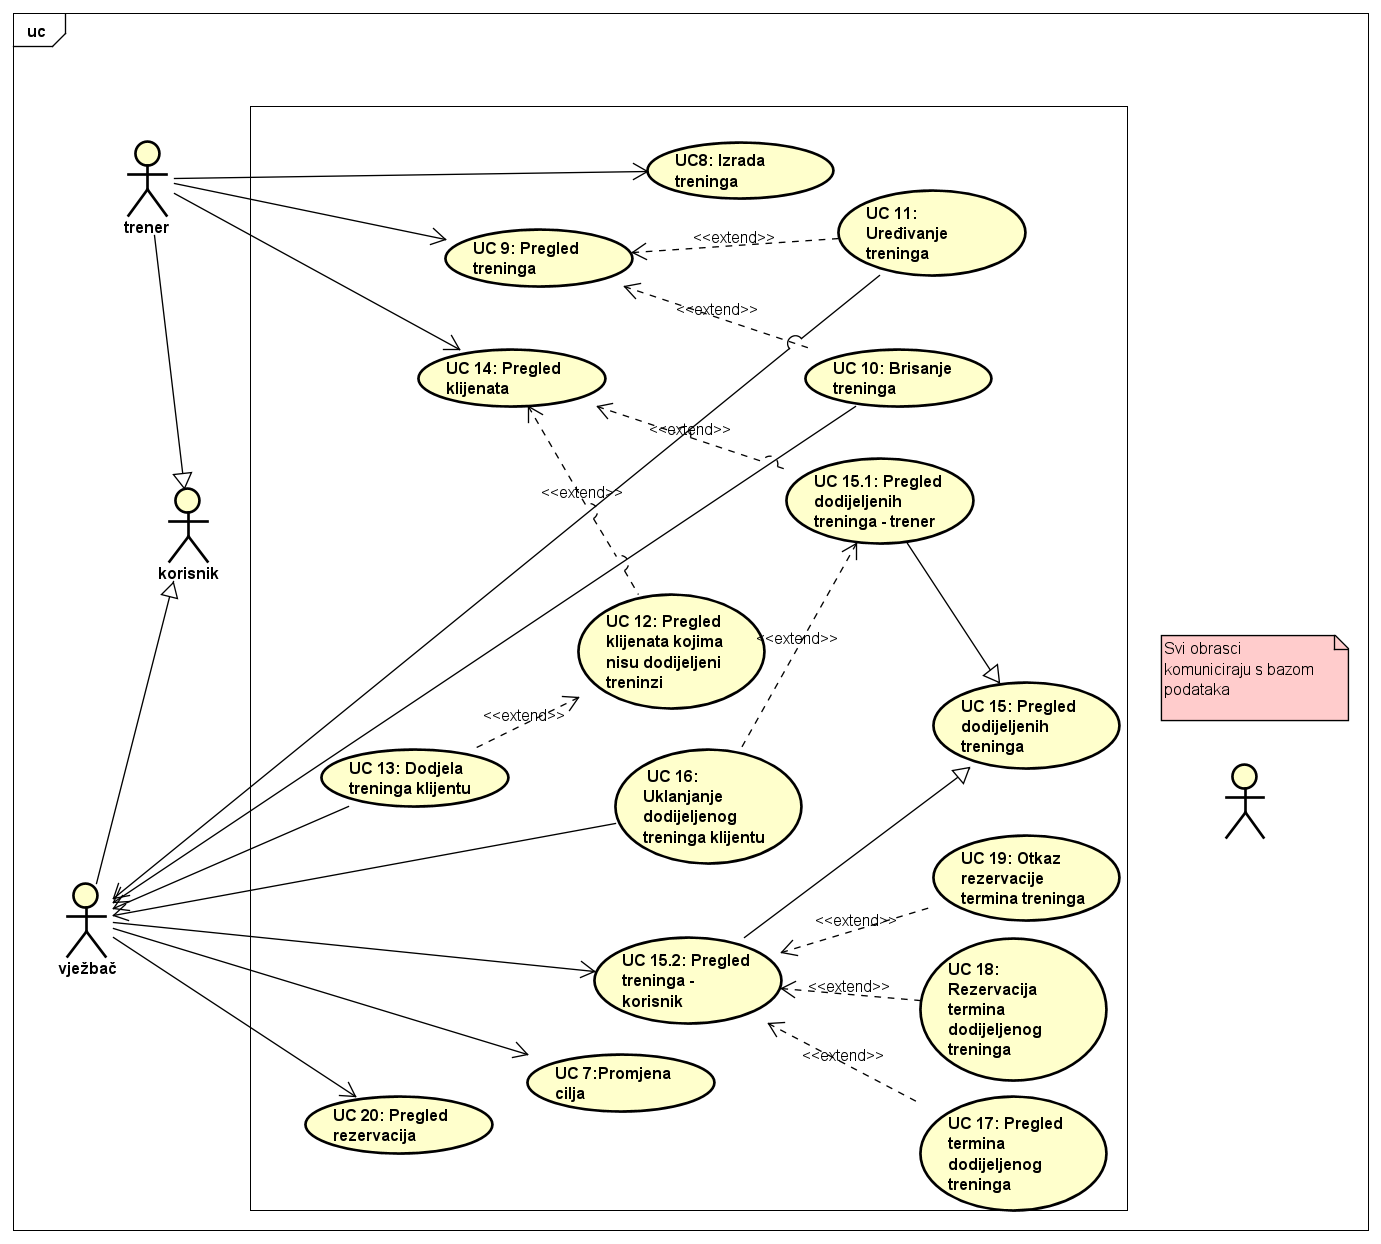
\includegraphics[scale=0.4]{./Dijagrami/UC1_Uloge.png}
                      \centering
                      \caption{Dijagram obrasca uporabe, funkcionalnost vježbača i trenera}
                      \label{fig:promjene}
                \end{figure}
                
				\eject		
				
			\subsection{Sekvencijski dijagrami}
   
	   			\subsubsection{Obrazac uporabe UC1: Registracija}
				\noindent Korisnik bira opciju za registraciju, te poslužitelj prikazuje formu za registraciju. Zatim korisnik unosi svoje ime, prezime, datum rođenja, e-mail adresu i broj telefona. Osmišlja korisničko ime i lozinku za prijavu, te odabire opciju želi li se registrirati kao vježbač ili kao trener. U slučaju da korisnik odabire opciju vježbač, odabire cilj. Po završetku ispunjavanja forme korisnik klikne na gumb registriraj se. Sustav provjerava dostupnost korisničkog imena, e-mail adrese, te ispravnost ostalih unesenih podataka u skladu sa zahtjevima sustava. Ukoliko su podaci ispravni, sustav šalje link za aktivaciju korisničkog računa na upisanu e-mail adresu i obavještava korisnika o uspješnoj registraciji. 

                \begin{figure}[H]
		              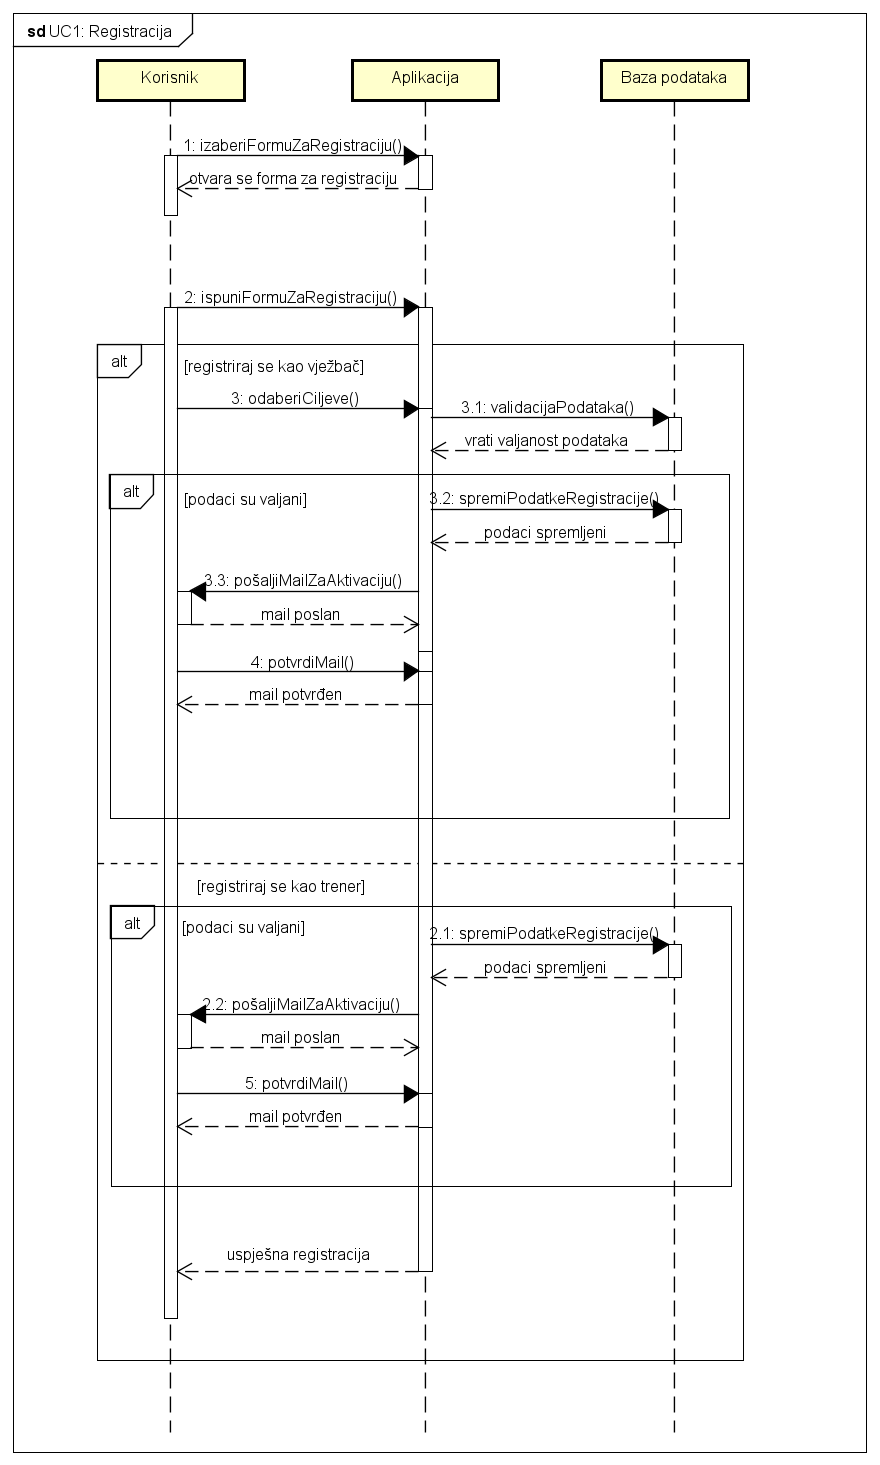
\includegraphics[scale=0.55]{./Dijagrami/UC1_Registracija.png}
		              \centering
		              \caption{Sekvencijski dijagram registracije}
		              \label{fig:promjene}
	            \end{figure}

                \subsubsection{Obrazac uporabe UC8: Izradi trening}
				\noindent Trener bira opciju "Izradi trening". Sustav otvara prozor za izradu treninga s formom za unos podataka o treningu. Trener unosi glavne podatke o treningu i odabire dane u tjednu u kojima bi se izvodio trening. Sustav za svaki dan nudi slobodne termine treninga koje zatim trener odabire za terning u izradi. Na kraju trener odabire opciju "Potvrdi", a sustav provjerava jesu li svi podaci ispravnog oblika. Ukoliko jesu sustav pohranjuje podatke o kreiranom treningu i njegovim terminima te ih sprema u bazu podataka. Ukoliko je sustav utvrdio da je trener unio neispravan oblik podataka o treningu, na zaslonu se pojavi poruka "Došlo je do pogreške".   

                \begin{figure}[H]
		              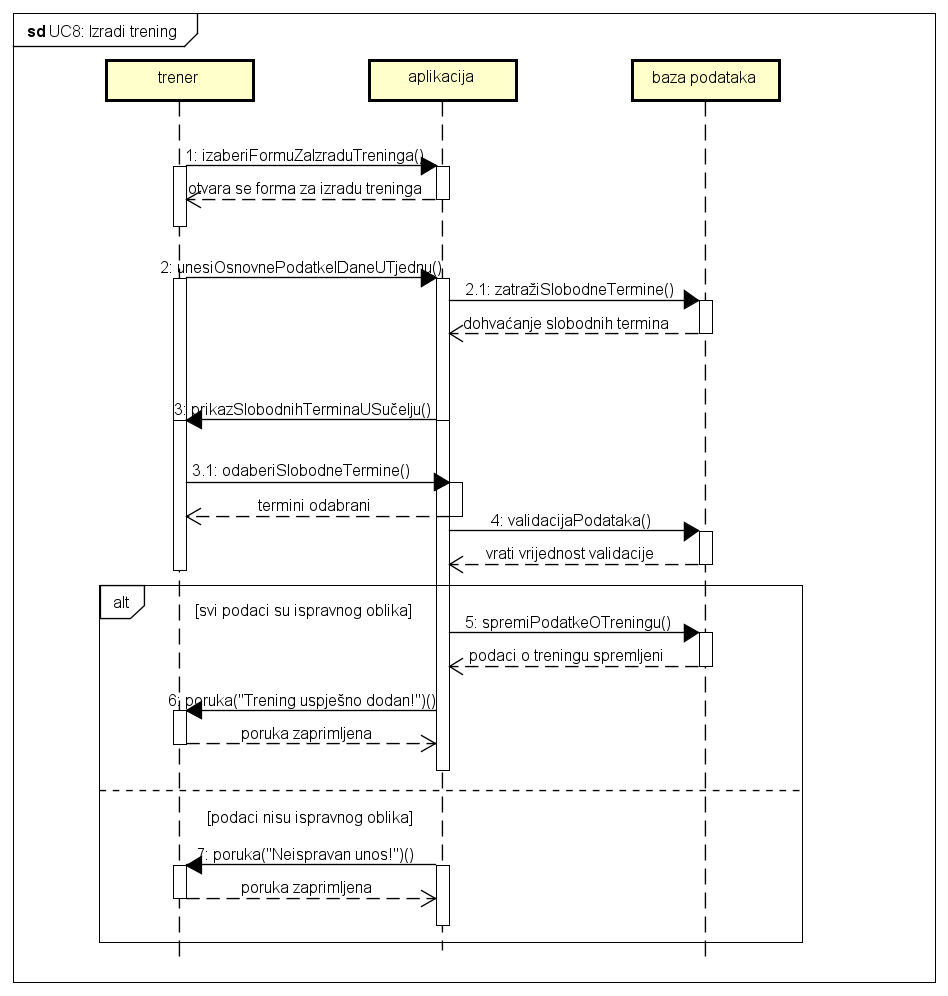
\includegraphics[scale=0.5]{./Dijagrami/UC8_Izradi_trening.png}
		              \centering
		              \caption{Sekvencijski dijagram izrade treninga}
		              \label{fig:promjene}
	            \end{figure}

                \subsubsection{Obrazac uporabe UC10: Dodjeli treninge klijentu}
				\noindent Trener klikom na gumb "Prikaz klijenata bez dodjeljenog treninga" otvara formu. Unutar te forme treneru se prikazuju svi mogući treninzi sa opcijom "Dodijeli". Treneru se odabirom opcije "Dodijeli" omogućuje i unos broja sati predviđenih za odrađivanje odabranih treninga. Trener potvrđuje odabrane treninge klikom na gumb "Spremi". Sustav ispituje ispravnost spremljenih podataka. Ukoliko su podaci ispravni, sustav sperma dodjeljene treninge i broj sati potrebnih da se oni odrade u bazu podataka. Zatim obavještava trenera o uspješno dodjeljenim treninzima iz sučelja aplikacije, a klijenta putem maila. Ukoliko podaci nisu ispravni aplikacija obavještava trenera o neuspješnom unosu treninga. 

                \begin{figure}[H]
		              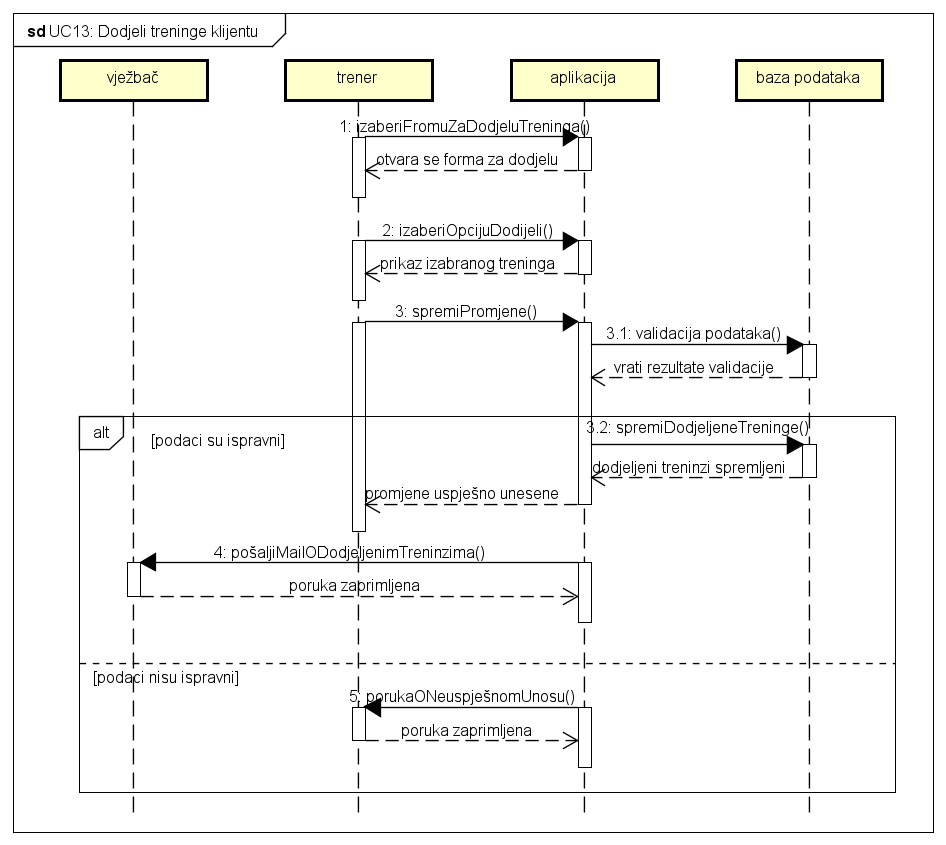
\includegraphics[scale=0.6]{./Dijagrami/UC13_Dodjeli_treninge_klijentu.png}
		              \centering
		              \caption{Sekvencijski dijagram dodjele treninga klijentima}
		              \label{fig:promjene}
	            \end{figure}

             
                \subsubsection{Obrazac uporabe UC12: Rezerviraj termin dodjeljenog treninga}
				\noindent Klijent ima pristup formi "Pregled dodjeljenih treninga". Klijent odabire termin među ponuđenima, a klikom na gumb "Rezerviraj" rezervira termin treninga. Sustav provjerava ograničenja. Ukoliko provjera odobrava rezervaciju treninga, aplikacija unosi podatak o rezervaciji u bazu podataka, smanjuje fond sati klijenta za jedan, smanjuje broj raspoloživim mjesta u rezervaciji treninga, i obavještava klijenta o uspješnoj rezervaciji u sučelju aplikacije. U slučaju neuspješne provjere sustav u sučelju aplikacije izdaje obavijest da rezervaciju nije moguće izvršiti zbog ograničenja.

                \begin{figure}[H]
		              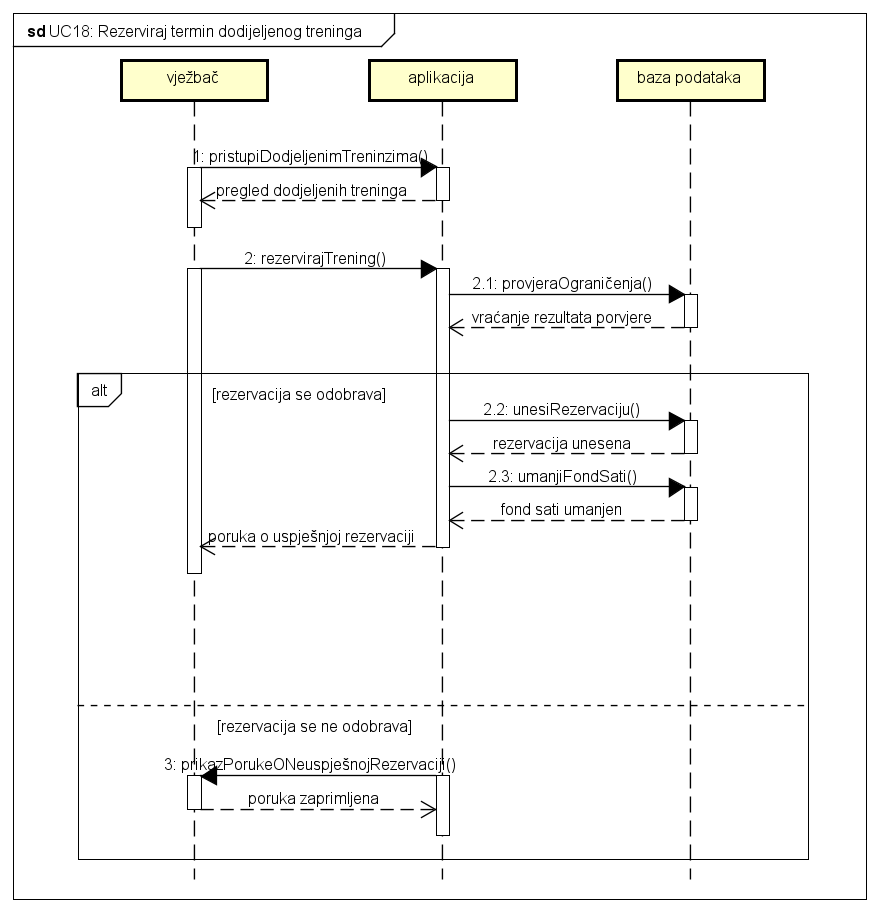
\includegraphics[scale=0.6]{./Dijagrami/UC18_ Rezerviraj_termin_dodijeljenog_treninga.png}
		              \centering
		              \caption{Sekvencijski dijagram rezervacije dodijeljenog termina}
		              \label{fig:promjene}
	            \end{figure}
               \eject
            
	
		\section{Ostali zahtjevi}
		
			%\textbf{\textit{dio 1. revizije}}\\
		 
			 {
			        Aplikacija treba biti izvedena kao web aplikacija kojoj će korisnici pristupati uz pomoć korisničkog imena i lozinke.\newline
                    Aplikacija treba biti jednostavna za korištenje, a sučelje pregledno i intuitivno. Osim toga, aplikacija treba biti prilagođena za rad na različitim uređajima (mobilni uređaj, tablet, PC).\newline
                    Aplikaciju treba implementirati u arhitekturi klijent-poslužitelj. Na poslužiteljskoj strani koristiti programski jezik Java i radni okvir Spring Boot, spremati podatke u relacijsku bazu podataka koristeći JPA, a potrebnu funkcionalnost izložiti kroz REST Web servise. \newline 
                    Na klijentskoj strani implementirati korisničko sučelje u Web pregledniku koristeći React ili Angular, koje se spaja na navedene servise.}
			 
			 
			 
	